\documentclass{beamer}

\usetheme[numbering=fraction,progressbar=foot]{custommoloch}

\usepackage[spanish,es-tabla]{babel}
\usepackage[utf8]{inputenc}

\title{Modelos Sencillos para Problemas Complejos}
\subtitle{Un Recorrido por el Ciclo del Dato \\
y la Evidencia del Mundo Real\\
en Medicina Personalizada}
\author{Carlos Loucera Muñecas}
\institute{Departamento de Ciencias de la Computación e Inteligencia Artificial}
\date{Escuela Técnica Superior de Ingeniería Informática, Sevilla, 04/05/2026}

\begin{document}
  \maketitle

  \begin{frame}{Contenido}
    \tableofcontents[hideallsubsections]
  \end{frame}

  \section[Camino]{El Camino hasta el CCIA}

    \begin{frame}{El Camino}
    \begin{figure}
        \includegraphics[width=0.99\textwidth]{figs/life/lou_life.pdf} 	
    \end{figure}
\end{frame}

\begin{frame}{Thesis}
	\begin{columns}
		\column{0.33\textwidth}

			\centering
			\begin{figure}
				\includegraphics[width=0.9\textwidth]{figs/camino/thesis/camino_thesis_virgen_foto.pdf}
			\end{figure}

			\pause

		\column{0.25\textwidth}

			\begin{figure}
				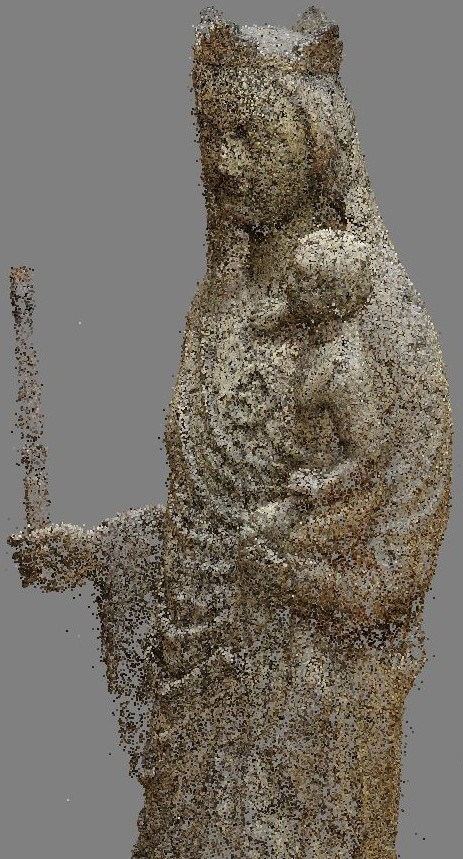
\includegraphics[width=0.9\textwidth]{figs/camino/thesis/camino_thesis_virgen_nube.jpg}
			\end{figure}

			\pause
		
		\column{0.42\textwidth}

			\begin{figure}
				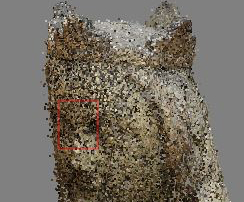
\includegraphics[width=0.7\textwidth]{figs/camino/thesis/camino_thesis_virgin_cropped.png} \\ 
				\pause
				\includegraphics[width=0.7\textwidth]{figs/camino/thesis/camino_thesis_virgen_filt_nose_crop.pdf}
			\end{figure}

	\end{columns}
\end{frame}

\begin{frame}{Automatic Defect Detection in Steam Generator Tubes}
	\begin{columns}
		\column{0.65\textwidth}

			\centering
			\begin{figure}
				\includegraphics[width=0.99\textwidth]{figs/camino/gtas/camino_gtas_diagram_etmachine.pdf}
			\end{figure}

			\pause

		\column{0.35\textwidth}

			\begin{figure}
				\includegraphics[width=0.99\textwidth]{figs/camino/gtas/camino_gtas_bien_emparejada.pdf}
			\end{figure}
	\end{columns}

	\vspace{\stretch{.5}}
	% vertically center logos with raisebox

	\raisebox{-0.5\height}{\includegraphics[width=2.5cm]{figs/camino/gtas/camino_gtas_logo_gtas.pdf}}
	\hspace{\stretch{1}}
	\raisebox{-0.5\height}{\includegraphics[width=3.5cm]{figs/camino/gtas/camino_gtas_logo_tecnatom.pdf}}
	\hspace{\stretch{1}}
	\raisebox{-0.5\height}{\includegraphics[width=0.8cm]{figs/camino/gtas/camino_gtas_logogran.pdf}}
	\hspace{\stretch{1}}
	\raisebox{-0.5\height}{
\includegraphics[width=3.5cm]{figs/camino/gtas/camino_gtas_seguridad_nuclear.png}}
\end{frame}


  \section[ER]{Reposicionamiento Computacional de Fármacos en Enfermedades Raras}

    
\begin{frame}{Rare Diseases 101}
	\begin{columns}
		\column{0.8\textwidth}
        Una ER afecta a \textbf{ 1 de cada 2000} personas. 
        
        Existen más de \textbf{7000 ERs distintas}.

        Se estima que el \textbf{6-8\%} de la población europea se ve afectada por al menos 1 enfermedad.
        
        \textbf{\textasciitilde 1 de cada 12} europeos se ve afectado

		\column{0.2\textwidth}

		\begin{figure}
			
\includegraphics[width=0.9\textwidth]{figs/er/rare-disease-logo.png}
		\end{figure}

	\end{columns}

	\pause

\begin{figure}
	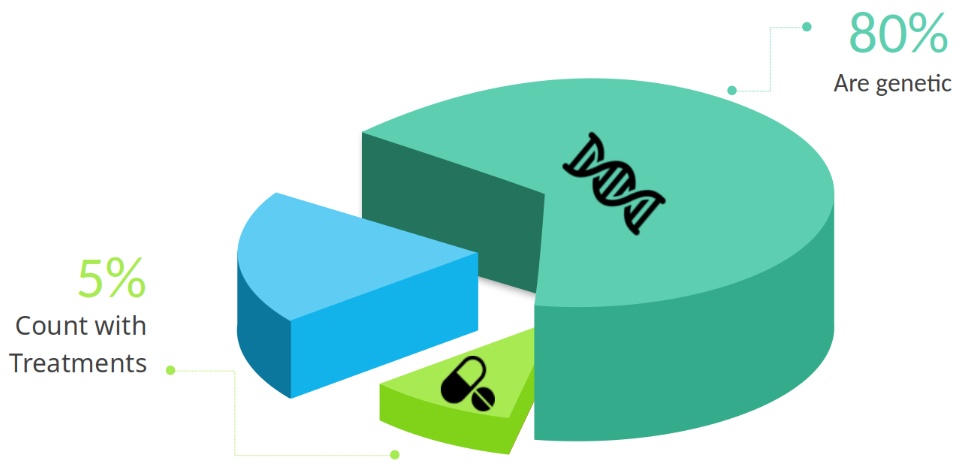
\includegraphics[width=0.7\textwidth]{figs/er/rare-disease-burden.png}
\end{figure}

\end{frame}


\begin{frame}{¿Por qué Reposicionamiento Computacional?}

    \renewcommand{\arraystretch}{1.8}
    \setlength{\arrayrulewidth}{3pt}
    \arrayrulecolor{white}

    \begin{adjustbox}{max width=\textwidth, max totalheight=0.82\textheight, keepaspectratio, center}
    \begin{tabular}{ p{2.8cm} p{6cm} p{6cm} }

        \rowcolor{headerblue}
        \textcolor{white}{\textbf{Dimensión}} &
        \textcolor{white}{\textbf{Reto}} &
        \textcolor{white}{\textbf{Solución computacional}} \\[2pt]

        \cellcolor{sideblue}\textcolor{white}{\textbf{Tratamiento}} &
        \cellcolor{headerblue!20} >7\,000 ERs con escasez de tratamientos &
        Fármacos aprobados reposicionados a nuevas indicaciones \\[2pt]

        \cellcolor{sideblue}\textcolor{white}{\textbf{Seguridad}} &
        \cellcolor{headerblue!20} Nuevos compuestos: perfil de riesgo desconocido &
        Perfil de seguridad y mecanismo de acción ya establecidos \\[2pt]

        \cellcolor{sideblue}\textcolor{white}{\textbf{Mecanismo}} &
        \cellcolor{headerblue!20} Relaciones fármaco-diana poco caracterizadas &
        Modelos mecanísticos de señalización celular \\[2pt]

        \cellcolor{sideblue}\textcolor{white}{\textbf{Datos}} &
        \cellcolor{headerblue!20} Escasez de muestras clínicas en ERs &
        Modelado funcional de la enfermedad desde BBDD $\rightarrow$ aprendizaje de perturbaciones en controles sanos \\[2pt]

        \cellcolor{sideblue}\textcolor{white}{\textbf{Escala}} &
        \cellcolor{headerblue!20} Miles de combinaciones fármaco-enfermedad &
        Aprendizaje automático $\cdot$ cMAP \\

    \end{tabular}
    \end{adjustbox}

\end{frame}

\begin{frame}{Reposicionamiento de fármacos 101}
	\centering
	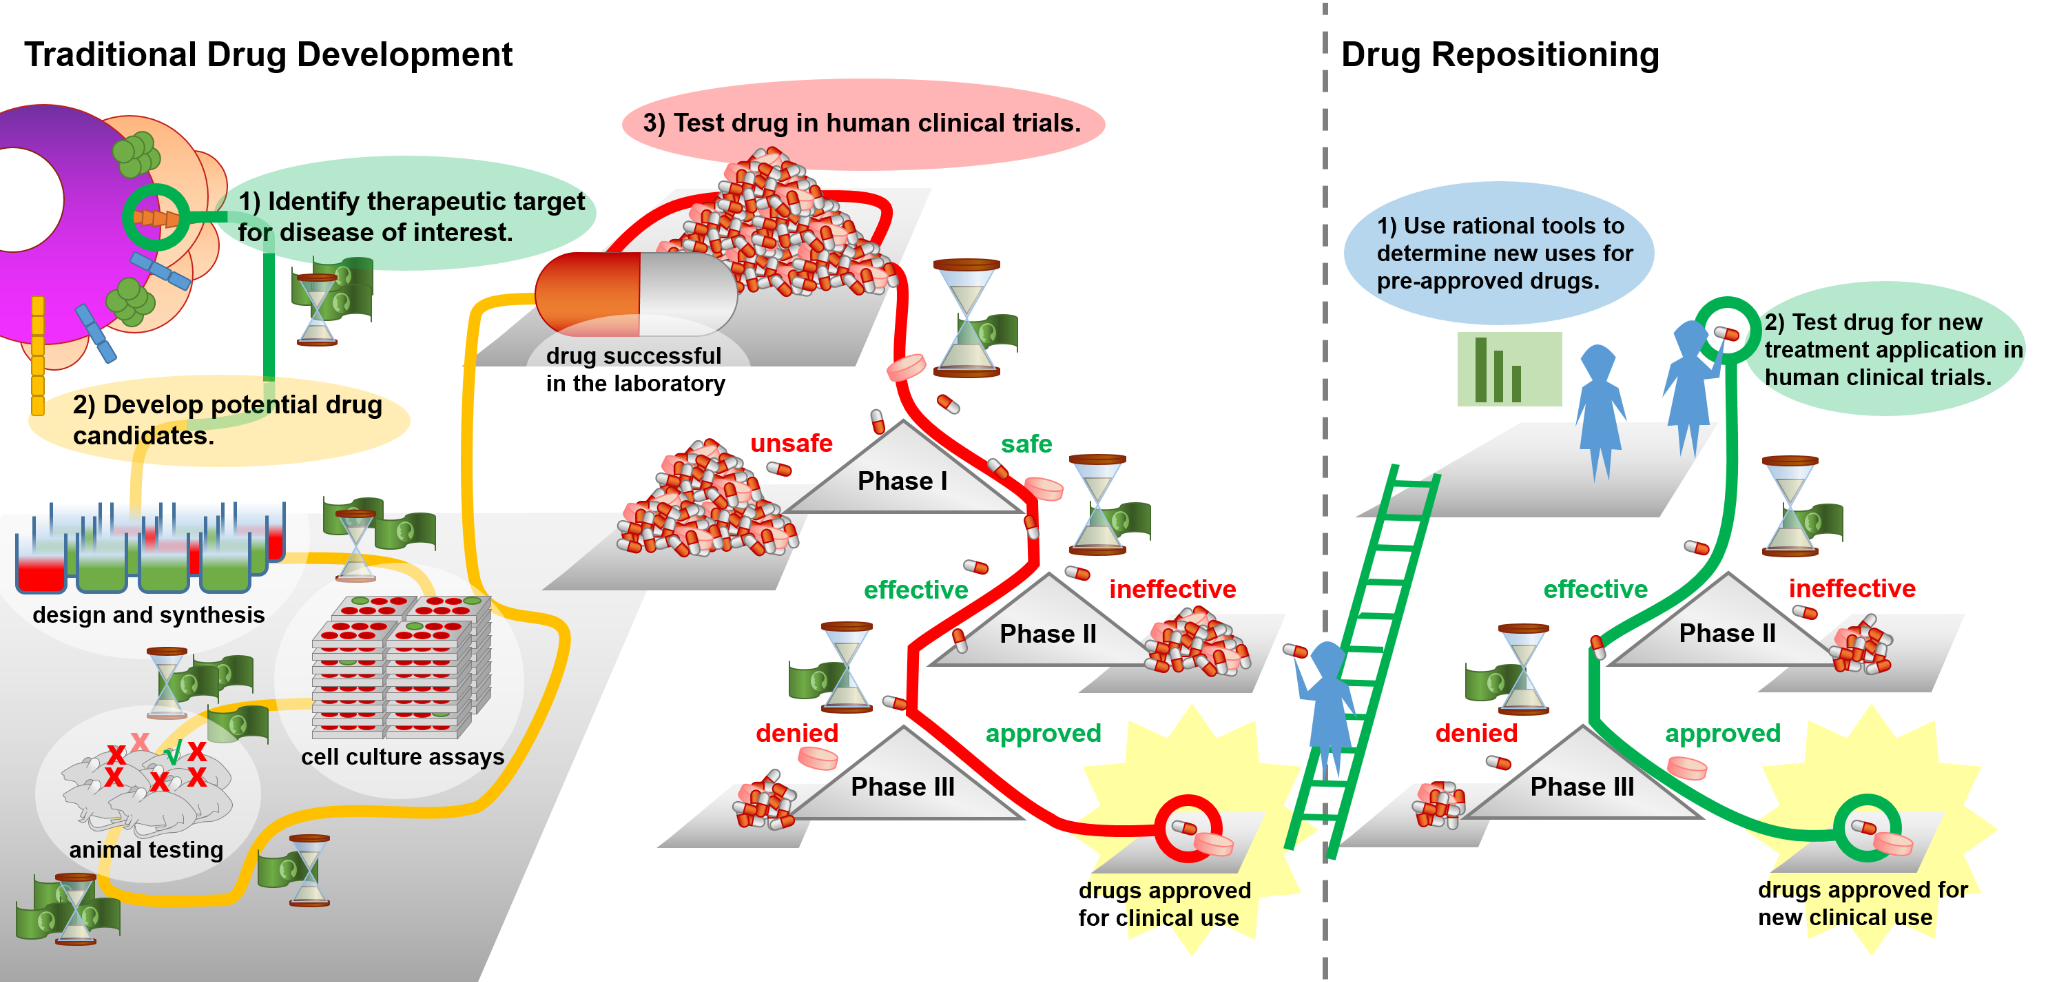
\includegraphics[width=\textwidth,height=0.82\textheight,keepaspectratio]{figs/er/repurposing-diagram.png}\\[2pt]
	{\fontsize{4}{5}\selectfont Fuente: \url{sitn.hms.harvard.edu/flash/2016/re-engineering-cures-big-data-age-precision-medicine-computational-drug-repositioning/}}
\end{frame}

\begin{frame}{Beneficios Coste Tiempo del Reposicionamiento}
	\centering
	\includegraphics[width=\textwidth,height=0.82\textheight,keepaspectratio]{figs/er/repurposing-cost-time.pdf}\\[2pt]
	{\fontsize{4}{5}\selectfont Fuente: \url{www.elsevier.com/industry/drug-repurposing}}
\end{frame}

\begin{frame}

	\begin{figure}
		\includegraphics[width=0.99\textwidth]{figs/er/repurposing-databases-step1.pdf}
	\end{figure}
	

\end{frame}

\begin{frame}

	\begin{figure}
		\includegraphics[width=0.99\textwidth]{figs/er/repurposing-databases-step2.pdf}
	\end{figure}
	

\end{frame}



  \section[]{}

\end{document}